

\section{Project management methodologies}
\label{ProjMgmtMethods}
This section details how the different teams manage themselves. This is done for reasons of transparency, so that the reader understands which project management methods the individual teams use. This highlights an additional level of complexity in the working environment. Not all teams are addressed in every subsection, as the project team was not involved in all teams’ methods to the same depth. First, project management methods are highlighted, followed by the different timeline management approaches. In the following figure, the different boards and management methods are aligned around the central academic team to illustrate the broad set of methods.


\begin{figure}[H]
    \centering
    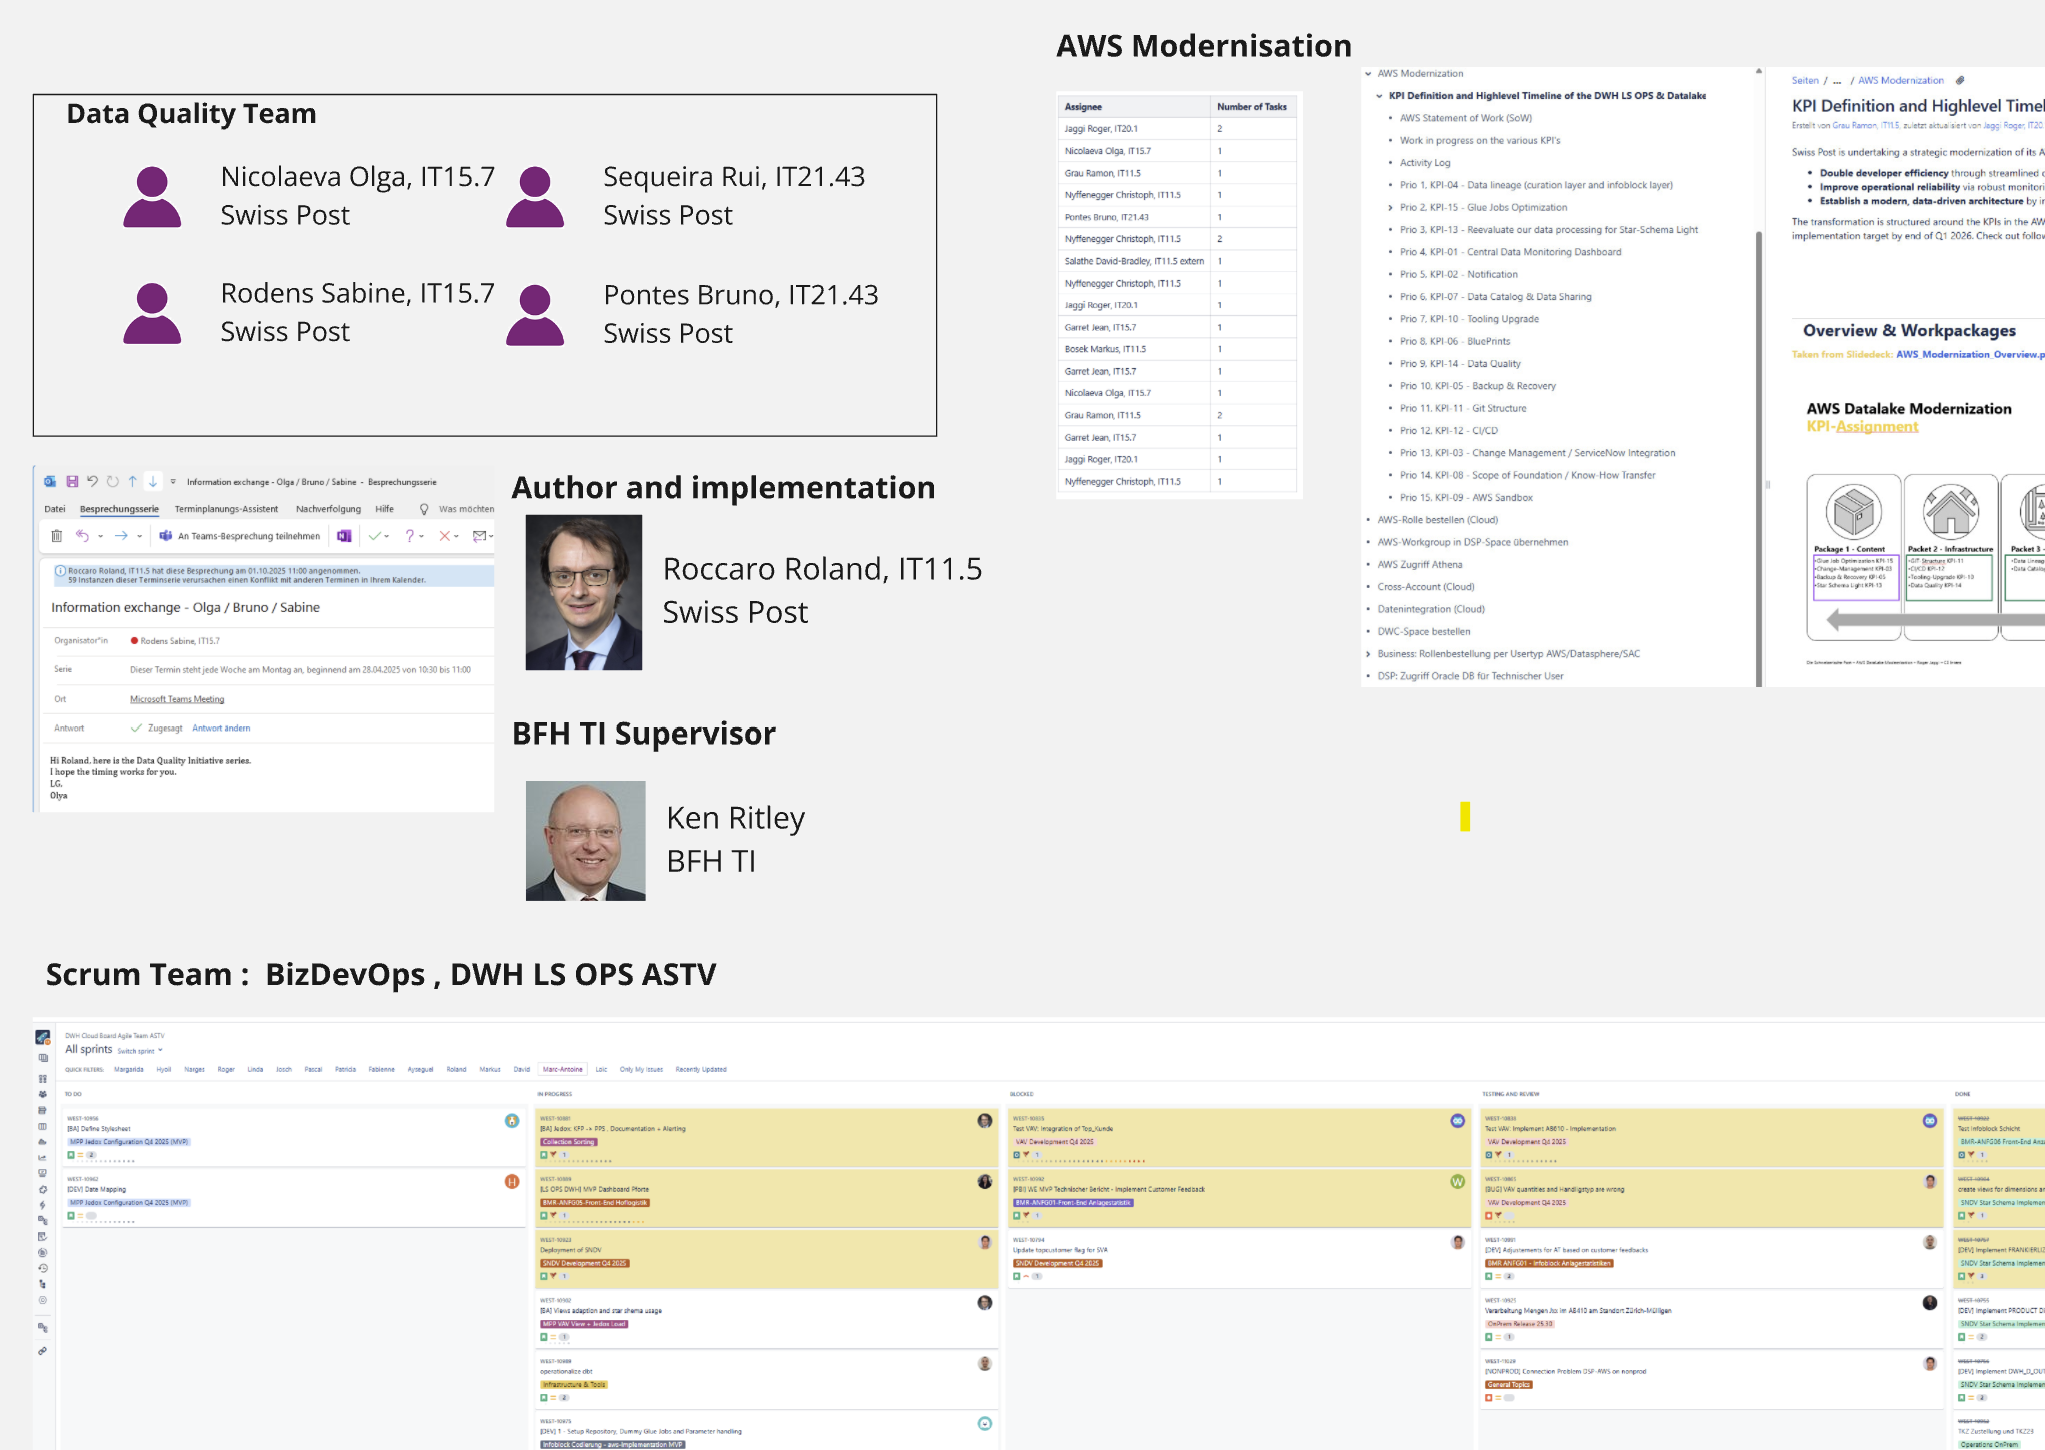
\includegraphics[width=0.8\textwidth]{./content/img/PostTeams_Tools.png}
    \caption{All methods shown in one figure. Top left: DQM team with weekly meetings. Top right: AWS modernisation using a Confluence page. Bottom: DWH LS OPS and academic team using Jira.}
    \label{fig:projmgmt_methods_one_pic}
\end{figure}


\subsection*{Project management}
Project management for this project consists of two main elements. These are Scrum and weekly meetings.

\subsubsection*{Scrum}
The \gls{DWHLSOPS} team is organised as a \gls{BizDevOps} \gls{scrum} team (see Section \ref{sec:DWHLSOPSTeam}). The AWS modernisation teams join these Scrum teams (see section \ref{sec:AWSmodernisationteam}). The full set of rituals defined for Scrum is used, including daily meetings, sprint retrospectives, sprint planning held every two weeks, and reviews held every four weeks. In addition, a weekly Scrum meeting is held to maintain communication between the ASTV, D\&F, and MPP teams. The meetings are shown in the first screenshot, while the second illustrates a noteworthy team definition: the rules of engagement established for collaboration, which are a result of the retrospectives.


\begin{figure}[H]
    \centering
    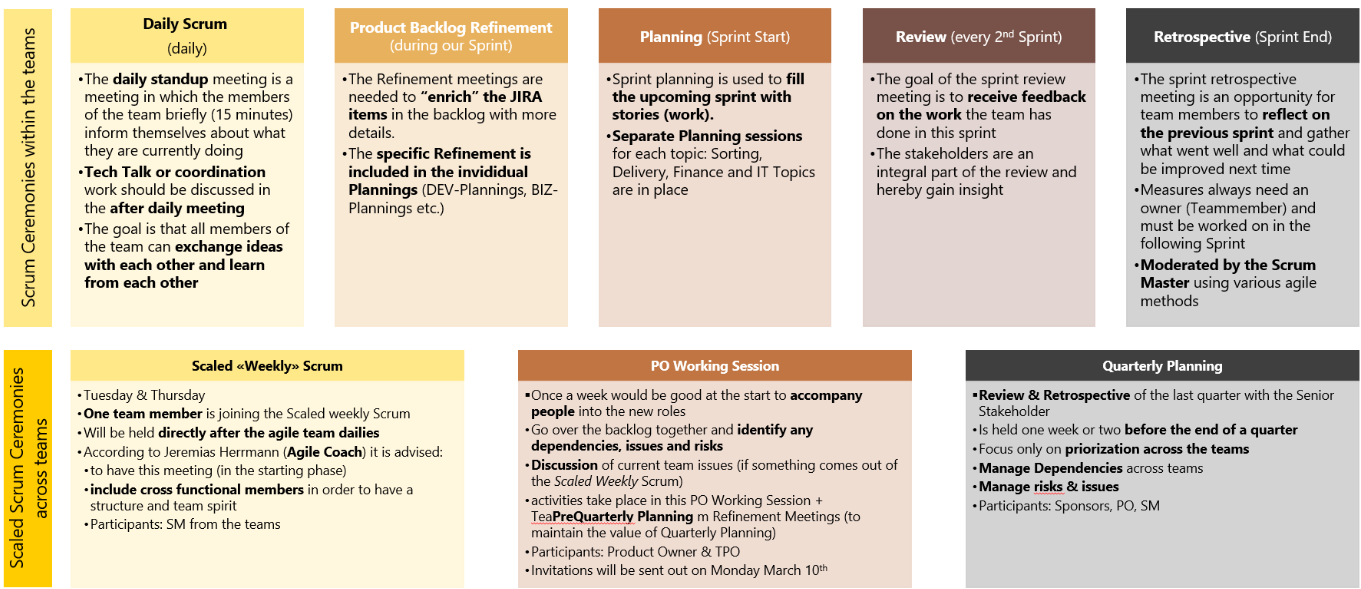
\includegraphics[width=0.8\textwidth]{./content/img/ProjectManagement/BizDevOps_ScrumCeremonies.PNG}
    \caption{Scrum ceremonies of DWH LS OPS  BizDevOps team}
    \label{fig:projmgmt_bizdevops_scrumMeetings}
\end{figure}

\begin{figure}[H]
    \centering
    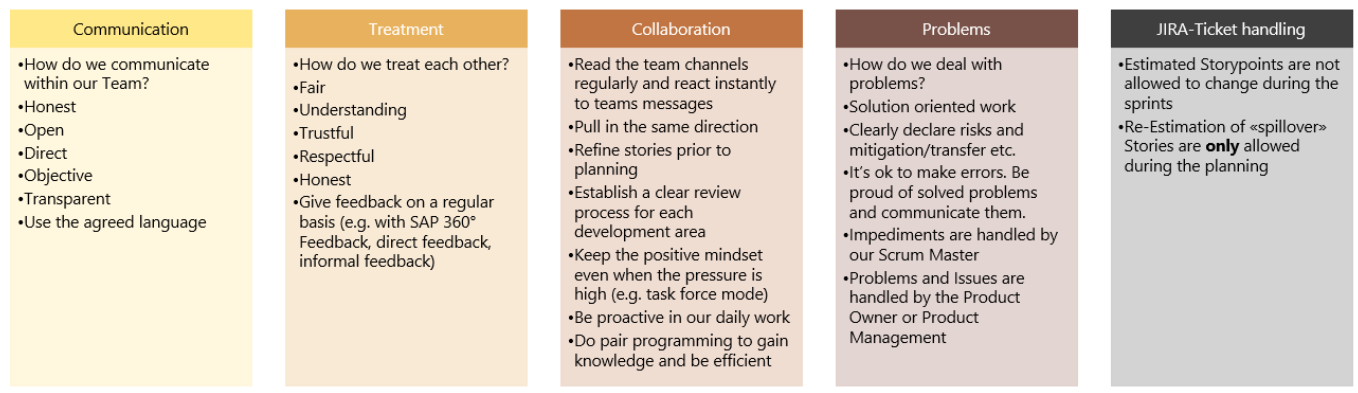
\includegraphics[width=0.8\textwidth]{./content/img/ProjectManagement/BizDevOps_RulesOfEngagement.png}
    \caption{Rules of engagement of DWH LS OPS  BizDevOps team}
    \label{fig:projmgmt_bizdevops_rulesofengagement}
\end{figure}

\subsubsection*{Weekly Meetings}
Contact with the \gls{DQM} team is handled through weekly meetings (see section \ref{sec:DQMteam}). These serve as minimal update sessions during which weekly progress is communicated to all team members. While the developers in the DQM team are themselves also part of a Scrum team, their sprint management is out of scope.

\subsubsection{Adapted Scrum}

The project team handles task planning and progress management using Scrum, however, in an adapted fashion. The DWH LS OPS board is used for a dual purpose. As a result, the sprint lengths are also two weeks. The board is linked to the shared Miro board for easier management within the academic team. The Scrum events are mainly held within the DWH LS OPS team. The academic team, however, performs a separate planning confirmation every two weeks and retrospectives, which happen less frequently. The dates for retrospectives are noted in the Miro calendar.



\subsubsection*{Jour Fixe}

The academic team holds a \gls{JourFixe} every week. This serves to maintain close communication and functions as a check-up meeting. Each meeting follows a defined structure; as an example, the meeting held on 12.10.2026 is described below.

\begin{itemize}
    \item Project check-in and clarification of objectives
    \item Overview of the project and completed deliverables
    \item Current deliverable in progress
    \item Update of initial project description
    \item Status of milestones
    \item Other topics
\end{itemize}

First, a general introduction to the project is provided to serve as a check-in and to allow participants to focus on the project. Second, the deliverables currently being worked on are listed based on the deliverables overview. Third, the status of the milestones is reviewed. Fourth, this is followed by individual agenda items, which can differ from meeting to meeting. In this meeting, these included updates to the initial project description, as well as a check-in regarding open administrative tasks such as handling contracts and payments. Finally, the meeting is closed with an open section in which any other relevant topics may be discussed. These meetings are documented in Miro (see below), structured using a three-block template, and most often recorded using handwritten notes that are later uploaded. Depending on the week's topics, some information, such as the sample below, is added. It shows the question of how to cite sources properly and the options provided.



 \begin{figure}[H]
    \centering
    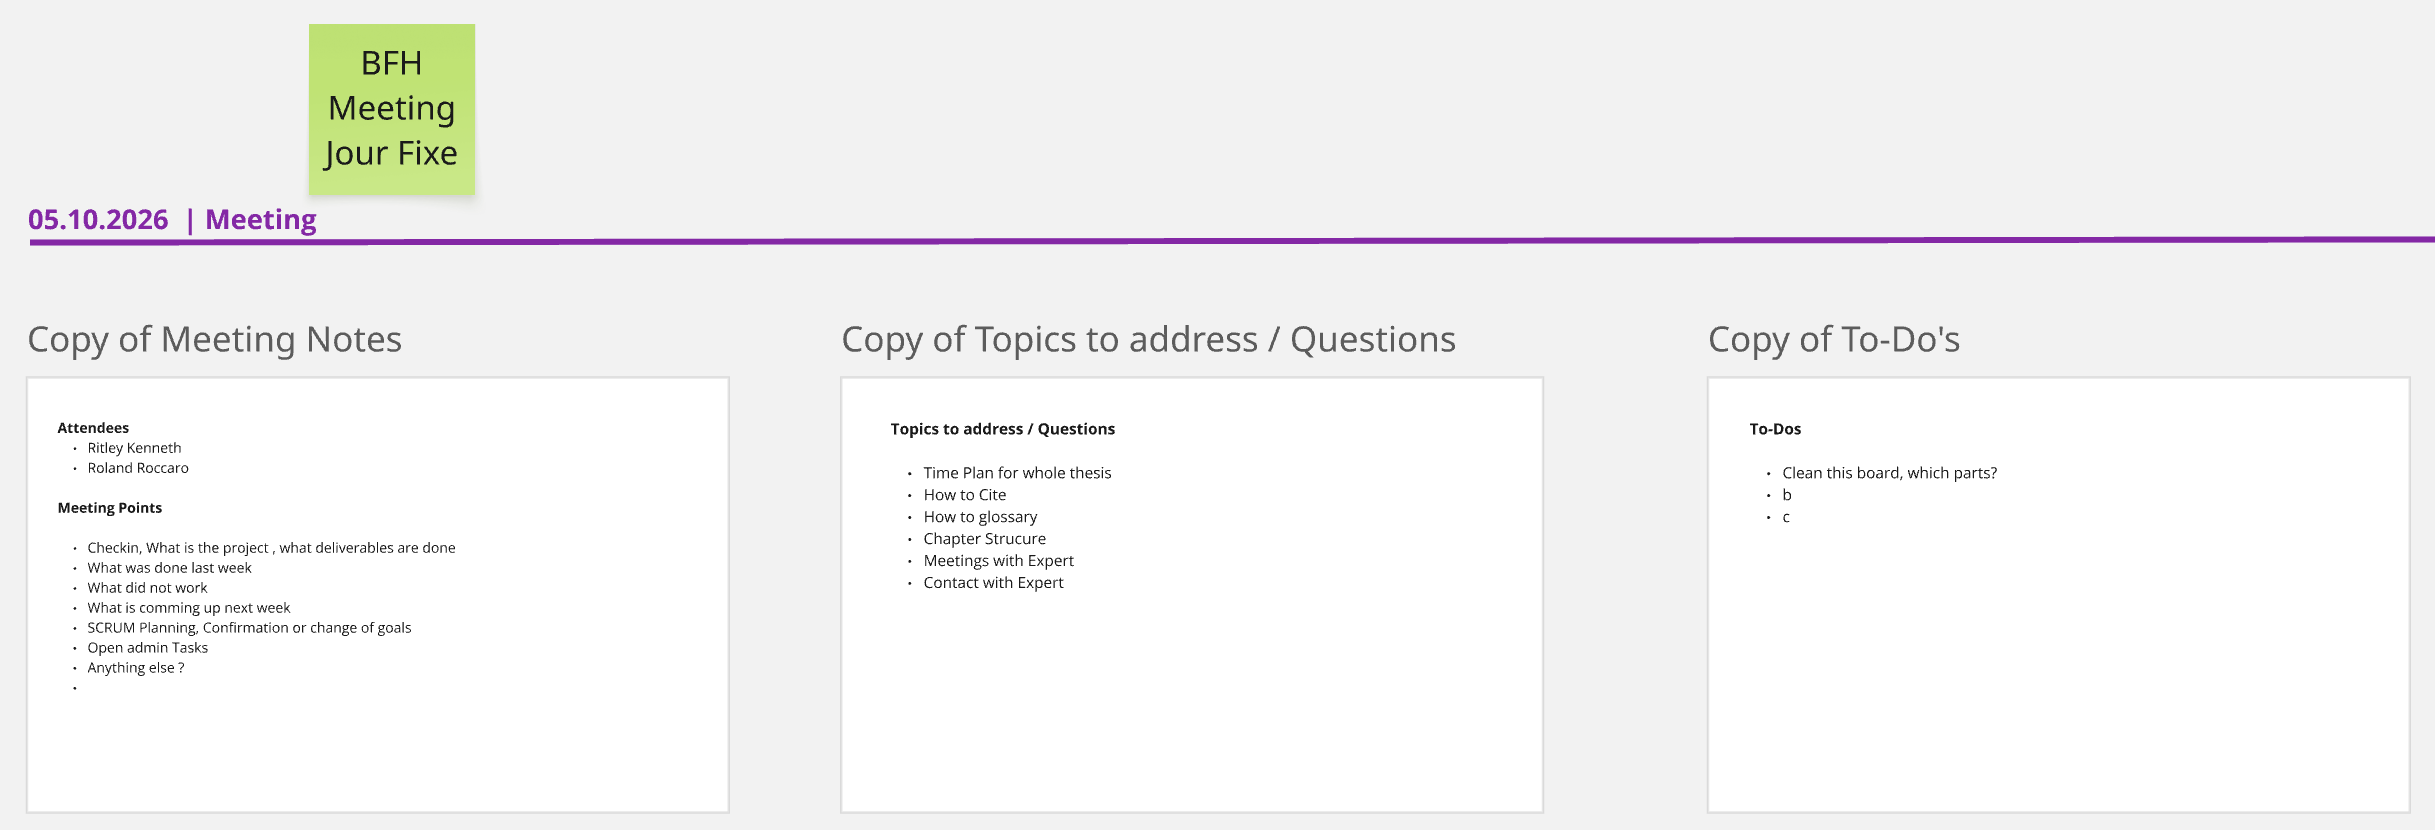
\includegraphics[width=0.8\textwidth]{./content/img/ProjectManagement/Academic_JourFixe.png}
    \caption{Jour Fixe of Academic team, meeting structure and rework}
    \label{fig:jour_fixe_academic_structure}
\end{figure}

\begin{figure}[H]
    \centering
    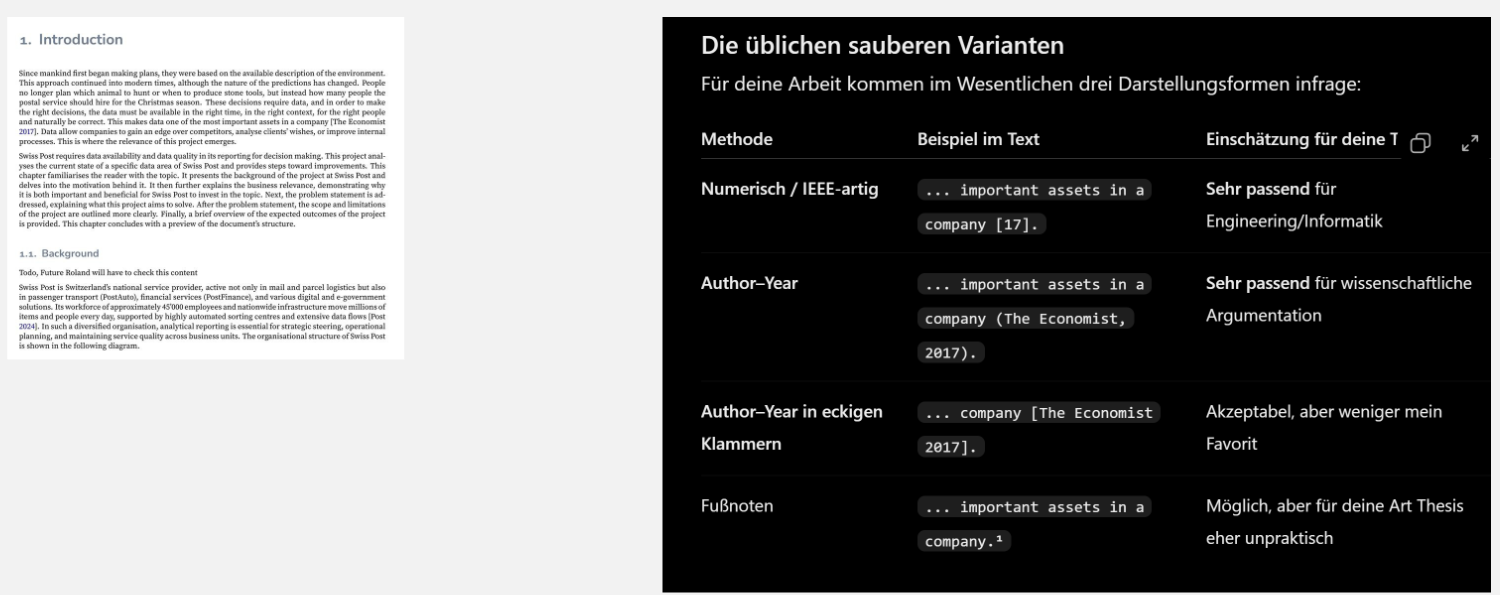
\includegraphics[width=0.8\textwidth]{./content/img/ProjectManagement/Academic_JourFixe_Pre_Notes.png}
    \caption{Jour Fixe documentation of the academic team. Example of a question to be discussed: How should citations be formatted, and is the current citation style appropriate?}
    \label{fig:jour_fixe_notes_academic}
\end{figure}

\subsection*{Timeline management}
Timeline management is performed in different ways by the teams. In this subsection, the planning of actions is described, as well as how staff availability is tracked.

\subsubsection*{Scrum Events}
All teams use Scrum events to manage their weekly progress. Progress on stories is monitored in daily meetings, during which each team member updates the team on progress and issues and indicates whether assistance is needed or deviations from the previously planned approach are required. Sprints encompass the stories the team works on during a two-week cycle. During sprint planning, the stories for the next sprint are defined. The stories added to a sprint represent the commitment the team makes for the sprint, together with the sprint goal. Planning over longer time horizons is conducted through quarterly planning sessions. Every three months, all teams in DWH LS OPS plan which \gls{epic}s should be completed and how many story points should be delivered. These quarterly planning sessions also serve to prioritise epics and allow higher management to introduce priorities.



\subsubsection*{Holidays}
Holidays are noted in the calendars used; this applies to the DWH LS OPS team as well as the academic team. In both cases, every holiday must be recorded with an absence notification. This allows other team members to quickly see whether a team member will be available in the future and to adjust their planning accordingly, or to confirm in daily operations that the person is not available.

\subsubsection*{Phases and milestones}
The academic team also uses phases and milestones to split the work into logical blocks and track its progress over the full duration. The details of these phases and milestones are described in their respective sections.

